\subsection{Discovering morphological categories}
\label{sec:categories}

A fundamental characteristic of words is that they belong to
part-of-speech categories such as nouns and verbs. Moreover, in
synthetic languages such as those we study, they carry inflectional
features such as number. We start by probing whether the
representations learned by our CNLM contains information about such
properties. We use here the popular model of ``diagnostic
classifiers'' \cite{Hupkes:etal:2017}. That is, we treat the hidden
activations produced by a CNLM whose weights were fixed after language model training as input features for a shallow (logistic)
classifier to distinguish the property of interest (e.g., plural
vs.~singular). If the classifier is successful, this means that the
representations provided by the model are encoding the relevant
information. In our case, we want to ask questions about word
properties to a model that has been trained at the character level. In
order to do that, we let the model read each training/test word
character-by-character, and we take the state of the model hidden
layer after having processed the last character in the word to be the
model's implicit representation of the word, on which we train the
diagnostic classifier. Note that the classifier is deliberately
shallow and trained on a small set of examples, as we want to probe
weather the properties of interests are robustly encoded in the
representations produced by the CNLMs, and amenable to a simple linear
readout \cite{Fusi:etal:2016}. %
% Besides being sensitive, to some extent, to word boundaries, does
% the CNLM also store linguistic properties of words, such as their part
% of speech and number?
The experiments focus on German and Italian, as it's harder to design
reliable test sets for morphologically impoverished English.

\paragraph{Word classes (nouns vs.~verbs)}

For both German and Italian, we sampled 500 verbs and 500 nouns from
the Wikipedia training sets, requiring that they are unambiguously
tagged in the corpus by TreeTagger. Since in many cases verbs and
nouns are cued by affixes, we selected the examples to have the same
ending across the two categories (\emph{-en} in German, e.g. \emph{Westen} `west'\footnote{German nouns are capitalized; this cue is unavailable to the CNLM as we lower-case the input.}% Just figured a reader might stumble over this, so added this footnote. Feel free to remove.
, \emph{stehen} `to stand'; and \emph{-re}
in Italian, e.g. \emph{autore} `author', \emph{dire} `to say'),
so that the models could not rely on affixes to
disambiguate the part of speech. We randomly selected 20 training
examples (10 nouns and 10 verbs), and tested on the remaining items.
We repeated the experiment 100 times to control for random train-test
split variation.
%  We recorded the final
% hidden state of a pre-trained CNLM after reading a word, without
% context, and trained a logistic noun-verb classifier on these
% representations.

While we controlled for the final affix as described above, it could
still be the case that other substrings reliably cue verbs or
nouns. In order to assess to what extent the models are relying on
information gathered from broader contexts, we consider a baseline
that is only trained on word-internal information. This is a
character-level LSTM autoencoder trained to reconstruct words in
isolation.  The hidden state of the autoencoder should capture
discriminating orthographic features, but, by design, the latter has
no access to broader contexts.  We further considered word embeddings
from the output layer of the WordNLM. Unlike the character-based
models, the WordNLM cannot make educated guesses about words that are
not in its training vocabulary. These OOV words are by construction
less frequent, and thus likely to be in general more difficult. To get
a sense of both ``best-case-scenario'' and more realistic WordNLM
performance, we report its accuracy both excluding and including OOV
items (WordNLM$_{\textit{subs.}}$ and WordNLM in Table
\ref{tab:pos-results}, respectively). In the latter case, we let the
model make a random guess for OOV items.  The percentage of OOV items
over the entire dataset, balanced for nouns and verbs, was 92.3\% for
German and 69.4\% for Italian.


Results are shown in Table~\ref{tab:pos-results}.  All language models
outperform the autoencoders, showing that they learned categories
based on broader distributional evidence, not just typical strings
cuing nouns and verbs. Moreover, the LSTM CNLM outperforms the RNN,
probably because it can track broader contexts. Not surprisingly, the
word-based model fares better on in-vocabulary words, but the gap,
especially in Italian, is rather narrow, and there is a strong
negative impact of OOV
words (as expected, as WordNLM must make random guesses here). % Figure~\ref{fig:pos-induction} shows how German performance evolves as the training set grows from 2 to 100 examples (Italian results are qualitatively identical). The CNLMs already distinguish the categories well with small training sets, while the autoencoder does not catch up even with 100 training examples per category.

\begin{table}[t]
%  \begin{small}
\footnotesize
    \begin{center}
      \begin{tabular}{l|l|l}
        &\emph{German}&\emph{Italian}\\
        \hline
        LSTM & 89.0 ($\pm$ 0.14) & 95.0 ($\pm$ 0.10) \\
        RNN & 82.0 ($\pm$ 0.64) & 91.9 ($\pm$ 0.24) \\
        Autoencoder & 65.1 ($\pm$ 0.22) & 82.8 ($\pm$ 0.26) \\
	      WordNLM$_{\textit{subs.}}$ & 97.4 ($\pm$ 0.05) & 96.0 ($\pm$ 0.06) \\
	      WordNLM & 53.5 ($\pm$ 0.18)  & 62.5 ($\pm$ 0.26) \\
      \end{tabular}
    \end{center}
 % \end{small}
	\caption{\label{tab:pos-results} Word class accuracy, with standard errors across 100 random train-test splits. `\emph{subs.}' marks in-vocabulary subset evaluation, not comparable to the other results.} % (20 training examples)
\end{table}


% \begin{figure}
% 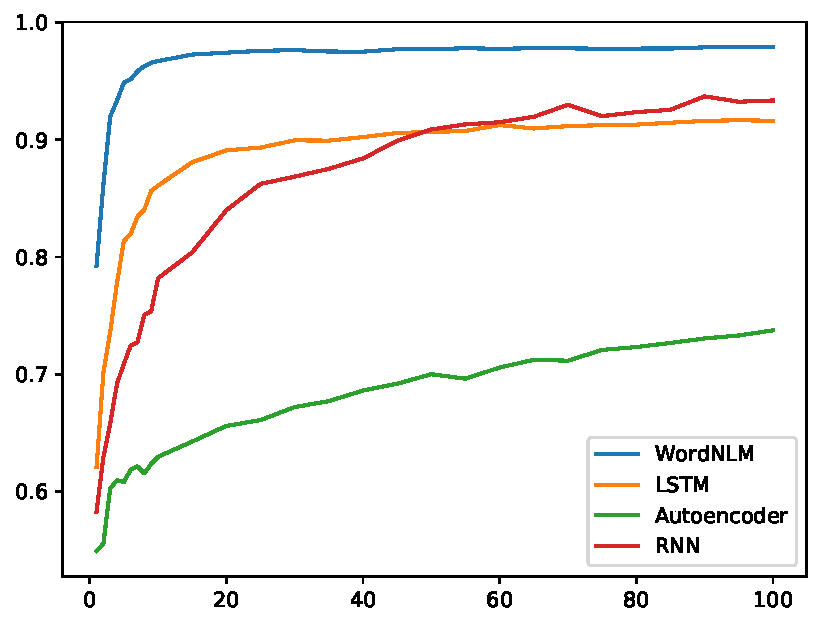
\includegraphics[width=0.48\textwidth]{figures/german_pos_nouns_verbs.pdf}
% 	\caption{Word class accuracy as a function of training examples (German). }\label{fig:pos-induction}
% 	% \textbf{Please rename LM LSTM, Baseline Autoencoder and Words WordNLM}
% \end{figure}




\paragraph{Number}
We turn next to number, a more granular morphological feature. We
study German, as it possesses a rich system of nominal classes forming
plural through different morphological processes. We train a diagnostic number
classifier on a subset of these classes, and test on the others. If a
model generalizes correctly, it means that the CNLM is sensitive to number
as an abstract feature, independently of its surface expression.

We extracted plural nouns from the Wiktionary and the German UD
treebank \cite{mcdonald2013universal,brants2002tiger}.  We
selected % de2006generating,
nouns with plurals in -\emph{n}, -\emph{s}, or -\emph{e} to train the
classifier (e.g., \emph{Geschichte-n} `stories' \textbf{MICHAEL:
  please also add examples of the other classes}), and tested on
plurals formed with -\emph{r} (e.g., \emph{Lieder} for singular
\emph{Lied} `song'), or through vowel change (\emph{Umlaut}, e.g.,
\emph{{\"A}pfel} for singular \emph{Apfel} `apple'). Certain nouns
form plurals through concurrent affixation and Umlaut (e.g.,
\textbf{MICHAEL: exmaple}). We grouped these together with nouns using
the same affix, reserving the Umlaut group for nouns \emph{only}
undergoing vowel change. \textbf{MICHAEL: can you add examples for all
  the classes, and for Umlaut pick an example not ending in -r (or
  other potential plural suffixes?).}

For the training set, we randomly selected 15 singulars and plurals
from each training class.  As plural suffixes make words longer, we
sampled singulars and
plurals %used rejection sampling \textbf{(cite something?)}
from a single distribution over lengths, to ensure that their lengths
were approximately matched. Moreover, since we observed that, in
uncontrolled samples from our training classes, \emph{-e-} as final
vowel would act as a strong surface cue to plurality, we controlled
the sampling to balance the distribution of this property across
singulars and plurals. For the test set, we selected all plurals
in -\emph{r} (127) or Umlaut (38), with their respective
singulars. %\textbf{(how many?)}.
We also used all remaining plurals ending in -\emph{n} (1467), -\emph{s} (98) and -\emph{e} (832) as in-domain test data.
%\textbf{Need information on the test set for the training classes.}
To control for the impact of training sample selection, we
report accuracies averaged over 200 random train-test splits and report standard errors over these splits.  We extract word
representations as above, and we compare the same models.
The percentage of singular-plural pairs where at least one of the two words were out of vocabulary for the WNLM was 63.4\% for the training classes, 68.6\% for -\emph{r} plurals, and 73.2\% for the Umlaut plurals.
Results are summarized in Table \ref{tab:number-results-e}.

The classifier based on word embeddings is the most successful,
outperforming in most cases the best CNLM even in the more cogent
OOV-inclusive evaluation. This confirms the common observation that
word embeddings reliably encode number \cite{Mikolov:etal:2013a}. The
CNLM results are mixed. Again the LSTM variant outperforms the
RNN, but neither has problems detecting number for new words from
the training paradigms. They are also able to detect number in a new
paradigm (\emph{-r} plurals), seemingly suggesting that they are, to some extent,
inducing an abstract notion of number that is not tied to specific
orthographic exponents. In these experiments, the CNLMs significantly
outperform the autoencoder. %, and the LSTM even does better than the
%word model in \emph{-r}-class generalization.

% We found that training classes tend to have an unstressed final -e- in
% the plural only, either as a plural ending (\emph{Abend} `evening' $\rightarrow$ \emph{Abend-e}) or as an epenthetic vowel
% intervening before a consonantal plural suffix (\emph{Autor} `author' $\rightarrow$ \emph{Autor-e-n}).
% However, all singulars
% that use only Umlaut to form their plurals have an unstressed final -e-
% in both singular and plural (e.g., \emph{Apfel} `apple' $\rightarrow$ \emph{{\"A}pfel}). 
% If the diagnostic classifier is sensitive to final unstressed -e- as a cue for plurals,
% it is expected that
% it should classify singulars and plurals as plurals.
% Indeed, we found that the CNLM classifiers mistook
% most Umlaut singulars for plurals.  On one randomly chosen split,
% 100\% of both singulars and plurals were classified as plurals.  
% No such problem occurs for -\emph{r} plurals, in contrast, as they
% follow the pattern of the training classes (e.g., \emph{Lied} `song' $\rightarrow$ \emph{Lied-e-r}).

% \textbf{Marco: Regarding your counterexamples (Kuss, Wurm), they fall under -e/-r plurals in the experiment. I clarified this at the beginning of this section.}

%By inspecting the results, we found that the CNLM classifiers mistook
%most Umlaut singulars for plurals.  On one randomly chosen split,
%100\% of both singulars and plurals were classified as plurals.  We
%observed that singulars using only Umlaut to mark plural have the
%commonality that their last vowel is an (unstressed) -\emph{e}-.  This
%vowel -\emph{e}- is also common in -\emph{r} plurals, many of which
%add a vowel -\emph{e}- between the consonant-final stem and the ending
%-\emph{r}.  Based on this observation, we hypothesized that the
%CNLM-based classifier detects the presence of -\emph{e}- towards the
%end of the word, which would explain why it does well on -\emph{r}
%plurals and at chance of Umlaut plurals. \textbf{MICHAEL: I think the
%  previous paragraph needs to be clarified in a few ways. First, it is
%  NOT always the case that Umlaut-triggering singulard have an
%  unstressed e as last vowel, Kuss, Wurm, etc. Do you mean that this
%  is the case in your data set? Then, this should be clarified (and
%  explained). Second, I think the argument would be clearer by turning
%  it around: Our training classes tend to have an unstressed final -e-
%  in the plural only. Many singulars in Umlaut have an unstressed
%  final -e-, hence the mishap. No problem with -r, as it follows the
%  pattern of the training classes. Finally, give examples!}

Performance of the diagnostic classifier for the LSTM CNLM is weaker than before for -\emph{r} plurals, and stronger than before for umlaut plurals.
That is, performance is weaker where the superficial cue used before (-\emph{e}-) was helpful (-\emph{r} plurals), and stronger where the cue is misleading (umlaut plurals).
%This is expected, as we had found that the performance in the first experiment could be explained mostly by presence of -\emph{e}-.
The autoencoder performs essentially at chance on held-out classes, showing that its previous modest success can be explained by the -\emph{e}- cue.
This shows that the CNLM encodes something more abstract than the autoencoder, but, overall, there is only modest evidence that the CNLM encodes any abstract notion of nominal plural in its hidden state.



\begin{table}[t]
	\footnotesize
  \begin{center}
    \begin{tabular}{@{\hspace{0.3em}}l@{\hspace{0.42em}}|@{\hspace{0.42em}}c@{\hspace{0.45em}}|@{\hspace{0.45em}}l@{\hspace{0.65em}}l@{\hspace{0.15em}}}
      &train classes&\multicolumn{2}{c}{test classes}\\
      &\emph{-n/-s/-e}&\multicolumn{1}{c}{\emph{-r}}&\multicolumn{1}{c}{\emph{Umlaut}}\\      \hline
	    LSTM & 71.5 ($\pm$ 0.8)  & 78.8 ($\pm$ 0.6)  & 60.8 ($\pm$ 0.6)  \\
	    RNN & 65.4 ($\pm$ 0.9)  & 59.8 ($\pm$ 1.0)  & 56.7 ($\pm$ 0.7)  \\
	    Autoencoder & 61.4 ($\pm$ 0.9)  & 50.7 ($\pm$ 0.8)  & 51.9 ($\pm$ 0.4)  \\
	    WordNLM$_{\textit{subs.}}$ & 97.1 ($\pm$ 0.3)  & 90.7 ($\pm$ 0.1)  & 97.5 ($\pm$ 0.1)  \\
	    WordNLM  & 77.3 ($\pm$ 0.7)  & 77.1 ($\pm$ 0.5)  & 74.2 ($\pm$ 0.6)  \\
    \end{tabular}
  \end{center}
  \caption{\label{tab:number-results-e} German number classification
	accuracy when controlling for -\emph{e}-, with standard errors computed from 200 random train-test
    splits.  `\emph{subs.}' marks in-vocabulary subset evaluation, not comparable to the other results.}
\end{table}


% PREVIOUS VERSION FROM HERE
% We turn next to number, a more granular morphological feature. We
% study German, as it possesses a rich system of nominal classes forming
% plural through different morphological processes. We train a diagnostic number
% classifier on a subset of these classes, and test on the others. If a
% model generalizes correctly, it means that the CNLM is sensitive to number
% as an abstract feature, independently of its surface expression.

% We extracted plural nouns from the Wiktionary and the German UD
% treebank \cite{mcdonald2013universal,brants2002tiger}.  We selected % de2006generating,
% nouns with plurals in -\emph{n}, -\emph{s}, or -\emph{e} to train the classifier (e.g., \emph{Geschichte-n} `stories'), and tested on plurals formed with
% -\emph{r} or through vowel change (\emph{Umlaut}, e.g., \emph{T{\"o}chter} for singular \emph{Tochter} `daughter'). \textbf{MICHAEL: maybe better to put also examples with -r, or at least not an Umlaut example ending in -r?}

% %\textbf{Add one
% %  example from training, one from testing.}

% For the training set, we randomly selected 15 singulars and plurals
% from each training class.  As plural suffixes make words longer, we
% sampled singulars and
% plurals %used rejection sampling \textbf{(cite something?)}
% from a single distribution over lengths, to ensure that their lengths
% were approximately matched.  For the test set, we selected all plurals
% in -\emph{r} (127) or Umlaut (38), with their respective
% singulars. %\textbf{(how many?)}.
% We also used all remaining plurals ending in -\emph{n} (1467), -\emph{s} (98) and -\emph{e} (832) as in-domain test data.
% %\textbf{Need information on the test set for the training classes.}
% To control for the impact of training sample selection, we
% report accuracies averaged over 200 random train-test splits and report standard errors over these splits.  We extract word
% representations as above, and we compare the same models. \textbf{MICHAEL: proportions of OOVs here.} %
% %, excluding OOVs when testing the latter.
% Results are summarized in Table \ref{tab:number-results}.

% \begin{table}[t]
% 	\footnotesize
%   \begin{center}
%     \begin{tabular}{@{\hspace{0.3em}}l@{\hspace{0.42em}}|@{\hspace{0.42em}}c@{\hspace{0.45em}}|@{\hspace{0.45em}}l@{\hspace{0.65em}}l@{\hspace{0.15em}}}
%       &train classes&\multicolumn{2}{c}{test classes}\\
%       &\emph{-n/-s/-e}&\multicolumn{1}{c}{\emph{-r}}&\multicolumn{1}{c}{\emph{Umlaut}}\\      \hline
% 	    LSTM & 73.5 ($\pm$ 0.7)  & 89.4 ($\pm$ 0.3)  & 53.7 ($\pm$ 0.3)  \\
% 	    RNN & 67.0 ($\pm$ 0.9)  & 83.5 ($\pm$ 0.5)  & 53.1 ($\pm$ 0.4)  \\
% 	    Autoencoder & 63.6 ($\pm$ 0.9)  & 78.1 ($\pm$ 0.5)  & 52.8 ($\pm$ 0.2)  \\
% 	    WordNLM$_{\textit{subs.}}$  & 97.4 ($\pm$ 0.3)  & 90.5 ($\pm$ 0.1)  & 97.3 ($\pm$ 0.1)  \\ 
% 	    WordNLM  & 78.2 ($\pm$ 0.7)  & 77.8 ($\pm$ 0.4)  & 75.9 ($\pm$ 0.5)  \\ 
%     \end{tabular}
%   \end{center}
%   \caption{\label{tab:number-results} German number classification
%     accuracy, with standard errors computed from 200 random train-test
%     splits.  `\emph{subs.}' marks in-vocabulary subset evaluation, not
%     comparable to the other results.}
% \end{table}

% % python char-lm-ud-stationary-separate-bidir-with-spaces-probe-baseline-prediction-wiki-plurals-2-tests-redone-wikisource.py --language german --batchSize 128 --char_embedding_size 100 --hidden_dim 1024 --layer_num 2 --weight_dropout_in 0.1 --weight_dropout_hidden 0.35 --char_dropout_prob 0.0 --char_noise_prob 0.01 --learning_rate 0.2 --load-from wiki-autoencoder

% % python char-lm-ud-stationary-separate-bidir-with-spaces-probe-baseline-prediction-wiki-plurals-2-tests-words-wikisource.py  --language german --batchSize 128 --char_embedding_size 200 --hidden_dim 1024 --layer_num 2 --weight_dropout_in 0.1 --weight_dropout_hidden 0.35 --char_dropout_prob 0.0 --char_noise_prob 0.01 --learning_rate 0.2 --load-from wiki-german-nospaces-bptt-words-966024846



% The classifier based on word embeddings is the most successful,
% outperforming in most cases the best CNLM even in the more cogent
% OOV-inclusive evaluation. This confirms the common observation that
% word embeddings reliably encode number \cite{Mikolov:etal:2013a}. The
% CNLM results are mixed. Again the LSTM variant outperforms the
% RNN, but neither has problems detecting number for new words from
% the training paradigms. They are also able to detect number in a new
% paradigm (\emph{-r} plurals), seemingly suggesting that they are, to some extent,
% inducing an abstract notion of number that is not tied to specific
% orthographic exponents. In these experiments, the CNLMs significantly
% outperform the autoencoder. %, and the LSTM even does better than the
% %word model in \emph{-r}-class generalization.

% In contrast, the CNLMs fail to generalize to Umlaut plurals, where
% they are virtually at chance level, similar to the autoencoder. %and \emph{worse} than the
% %autoencoder.
% % The most obvious difference between this type and
% % \emph{-r} pluralization is that the latter is an affixation process,
% % whereas Umlaut pluralization changes the stressed vowel of the
% % stem.
% By inspecting the results, we found that the CNLM classifiers mistook
% most Umlaut singulars for plurals.  On one randomly chosen split,
% 100\% of both singulars and plurals were classified as plurals.  We
% observed that singulars forming their plural with Umlaut have the
% commonality that their last vowel is an (unstressed) -\emph{e}-.  This
% vowel -\emph{e}- is also common in -\emph{r} plurals, many of which
% add a vowel -\emph{e}- between the consonant-final stem and the ending
% -\emph{r}.  Based on this observation, we hypothesized that the
% CNLM-based classifier detects the presence of -\emph{e}- towards the
% end of the word, which would explain why it does well on -\emph{r}
% plurals and at chance of Umlaut plurals. \textbf{MICHAEL: I think the
%   previous paragraph needs to be clarified in a few ways. First, it is
%   NOT always the case that Umlaut-triggering singulard have an
%   unstressed e as last vowel, Kuss, Wurm, etc. Do you mean that this
%   is the case in your data set? Then, this should be clarified (and
%   explained). Second, I think the argument would be clearer by turning
%   it around: Our training classes tend to have an unstressed final -e-
%   in the plural only. Many singulars in Umlaut have an unstressed
%   final -e-, hence the mishap. No problem with -r, as it follows the
%   pattern of the training classes. Finally, give examples!}

% To test this hypothesis, we created a na\"ive ``classifier'' that
% labels a word as plural if one of the last two characters is \emph{e}.
% On the full dataset, this classification method achieves 73.7 \%
% accuracy on the train classes, 95.1\% on -\emph{r} plurals, and 51.0\%
% on Umlaut plurals.  This accuracy is close to that of the LSTM CNLM on
% in-domain and Umlaut, and even outperforms it on -\emph{r}.  Across
% the 200 runs, average agreement between classification decisions made
% with this simple heuristic and the CNLM-based ones was 75.0\%
% ($\pm$0.8) on the in-domain classes, 89.5 ($\pm$ 0.3) on the
% -\emph{r}, and 95.4 ($\pm$0.4) on Umlaut.  We conclude that, in the
% experiment described above, the CNLM classifier was strongly
% influenced by a very superficial cue (presence of -\emph{e}- near the
% word end) that correlates with plural-hood reasonably well, but does
% not generalize well across morphological classes of plural formation.

% % python char-lm-ud-stationary-separate-bidir-with-spaces-probe-baseline-prediction-wiki-plurals-2-tests-redone-wikisource-investigateE.py --language german --batchSize 128 --char_embedding_size 100 --hidden_dim 1024 --layer_num 2 --weight_dropout_in 0.1 --weight_dropout_hidden 0.35 --char_dropout_prob 0.0 --char_noise_prob 0.01 --learning_rate 0.2 --load-from wiki-german-nospaces-bptt-910515909

% Informed by this result, we repeated the experiment with controlled
% training sets where incidence of -\emph{e}- was balanced across
% singulars and plurals.  To balance for the plurals, we made sure that
% 1/4 of those ending in -r or -s had an -\emph{e}- as their
% second-to-last character, so that the total fraction of training
% plurals with -\emph{e}- in the last two characters was 1/2.  For
% singulars, we balanced the incidence of -\emph{e}- for each of the
% classes.  Resulting accuracies are shown in
% Table~\ref{tab:number-results-e}.

% Performance of the diagnostic classifier for the LSTM CNLM is weaker than before for -\emph{r} plurals, and stronger than before for umlaut plurals.
% That is, performance is weaker where the superficial cue used before (-\emph{e}-) was helpful (-\emph{r} plurals), and stronger where the cue is misleading (umlaut plurals).
% %This is expected, as we had found that the performance in the first experiment could be explained mostly by presence of -\emph{e}-.
% The autoencoder performs essentially at chance on held-out classes, showing that its previous modest success can be explained by the -\emph{e}- cue.
% This shows that the CNLM encodes something more abstract than the autoencoder, but, overall, there is only modest evidence that the CNLM encodes any abstract notion of nominal plural in its hidden state.



% \begin{table}[t]
% 	\footnotesize
%   \begin{center}
%     \begin{tabular}{@{\hspace{0.3em}}l@{\hspace{0.42em}}|@{\hspace{0.42em}}c@{\hspace{0.45em}}|@{\hspace{0.45em}}l@{\hspace{0.65em}}l@{\hspace{0.15em}}}
%       &train classes&\multicolumn{2}{c}{test classes}\\
%       &\emph{-n/-s/-e}&\multicolumn{1}{c}{\emph{-r}}&\multicolumn{1}{c}{\emph{Umlaut}}\\      \hline
% 	    LSTM & 71.5 ($\pm$ 0.8)  & 78.8 ($\pm$ 0.6)  & 60.8 ($\pm$ 0.6)  \\
% 	    RNN & 65.4 ($\pm$ 0.9)  & 59.8 ($\pm$ 1.0)  & 56.7 ($\pm$ 0.7)  \\
% 	    Autoencoder & 61.4 ($\pm$ 0.9)  & 50.7 ($\pm$ 0.8)  & 51.9 ($\pm$ 0.4)  \\
% 	    WordNLM$_{\textit{subs.}}$ & 97.1 ($\pm$ 0.3)  & 90.7 ($\pm$ 0.1)  & 97.5 ($\pm$ 0.1)  \\
% 	    WordNLM  & 77.3 ($\pm$ 0.7)  & 77.1 ($\pm$ 0.5)  & 74.2 ($\pm$ 0.6)  \\
%     \end{tabular}
%   \end{center}
%   \caption{\label{tab:number-results-e} German number classification
% 	accuracy when controlling for -\emph{e}-, with standard errors computed from 200 random train-test
%     splits.  `\emph{subs.}' marks in-vocabulary subset evaluation, not comparable to the other results.}
% \end{table}

% PREVIOUS VERSION TO HERE

% python char-lm-ud-stationary-separate-bidir-with-spaces-probe-baseline-prediction-wiki-plurals-2-tests-words-wikisource-balanceE.py  --language german --batchSize 128 --char_embedding_size 200 --hidden_dim 1024 --layer_num 2 --weight_dropout_in 0.1 --weight_dropout_hidden 0.35 --char_dropout_prob 0.0 --char_noise_prob 0.01 --learning_rate 0.2 --load-from wiki-german-nospaces-bptt-words-966024846

% python char-lm-ud-stationary-separate-bidir-with-spaces-probe-baseline-prediction-wiki-plurals-2-tests-redone-wikisource-balanceE.py --language german --batchSize 128 --char_embedding_size 100 --hidden_dim 1024 --layer_num 2 --weight_dropout_in 0.1 --weight_dropout_hidden 0.35 --char_dropout_prob 0.0 --char_noise_prob 0.01 --learning_rate 0.2 --load-from wiki-german-nospaces-bptt-910515909

% python char-lm-ud-stationary-separate-bidir-with-spaces-probe-baseline-prediction-wiki-plurals-2-tests-redone-wikisource-balanceE-RNN.py --batchSize 256 --char_dropout_prob 0.01 --char_embedding_size 50 --char_noise_prob 0.0 --hidden_dim 2048 --language german --layer_num 2 --learning_rate 0.1 --lr_decay 0.95 --nonlinearity tanh --load-from wiki-german-nospaces-bptt-rnn-237671415 --sequence_length 30 --verbose True --weight_dropout_hidden 0.0 --weight_dropout_in 0.0

% python char-lm-ud-stationary-separate-bidir-with-spaces-probe-baseline-prediction-wiki-plurals-2-tests-words-wikisource-balanceE-withOOV.py  --language german --batchSize 128 --char_embedding_size 200 --hidden_dim 1024 --layer_num 2 --weight_dropout_in 0.1 --weight_dropout_hidden 0.35 --char_dropout_prob 0.0 --char_noise_prob 0.01 --learning_rate 0.2 --load-from wiki-german-nospaces-bptt-words-966024846






 













%Thus, a cautious interpretation is that the CNLMs developed a
%representation of plural that is sufficiently abstract to generalize
%to different affixation processes than the ones seen in training,
%but. Note that, as we control for length, we are confident that the
%network is not simply relying on this superficial feature to detect
%plurals (which would explain why affixation cases are
%easier). Similarly, the network can't simply rely on consonants cuing
%plurals, both because many singular forms also end with consonants, and
%because one of the training classes had \emph{-e} as plural marker.
%\textbf{We need some kind of story here!!!}
%% Evidently, CNLM number encoding is not abstract enough to
%% generalize across very different surface morphological processes
%% (adding a suffix vs.~changing the root vowel).
%
%Interestingly, many of the Umlaut words end in \emph{-n} and \emph{-r}, and these singulars are mostly misclassified as plurals. 
%We hypothesized that the CNLMs-based classifiers classify number based on the orthographic endings, not based on abstract number representations.
%To test this, we extracted from Wiktionary singular nouns ending in \emph{-n, -s, -e, -r}, excluding nouns that have identical singular and plural forms.
%We also extracted nouns ending in one of the two most common final characters of singular nouns in the dataset that can \emph{not} act as the last character of a plural, which are \emph{g} and \emph{t}.
%We then ran the number classifier on these nouns, again with 200 random choices of the training set.

%Resulting accuracies are shown in Table~\ref{tab:number-foils-results}.
%Classifiers based on CNLM or autoencoder representations show relatively poor accuracies on the singulars ending in characters typical of plurals (\emph{-n, -s, -e, -r}), i.e., the diagnostic classifiers mistake many singulars for plurals based on their ending.
%Conversely, they mostly recognize singulars when the final consonant makes this unambiguous.
%This suggests that -- to the extent accessible to a shallow diagnostic classifier -- the CNLM encodes not an abstract number feature, but orthographic features typical of plurals.
%
%\begin{table}[t]
%	\footnotesize
%  \begin{center}
%    \begin{tabular}{@{\hspace{0.3em}}l@{\hspace{0.42em}}|@{\hspace{0.42em}}c@{\hspace{0.45em}}@{\hspace{0.45em}}l@{\hspace{0.65em}}|l@{\hspace{0.15em}}}
%	    &\emph{-n}/\emph{-s}/\emph{-e}&\emph{-r}&\emph{-g}/\emph{-t}  \\ \hline
%	    LSTM& 65.2 ($\pm$ 0.7)  & 55.1 ($\pm$ 0.2) & 83.2 ($\pm$ 0.4) \\
%	    RNN& 61.3 ($\pm$ 0.2) &  51.6 ($\pm$ 0.2) & 75.5 ($\pm$ 0.1) \\
%	    Autoencoder& 65.7 ($\pm$ 0.3) & 50.0 ($\pm$ 0.2) & 72.5 ($\pm$ 0.2) \\
%	    WordNLM$_{\textit{subs.}}$& 93.4 ($\pm$ 0.1) & 95.2 ($\pm$ 0.3) & 93.3 ($\pm$ 0.2) \\
%	    WordNLM & 86.3 ($\pm$ 0.1) & 88.8 ($\pm$ 0.2) & 88.4 ($\pm$ 0.3) \\
%    \end{tabular}
%  \end{center}
%	\caption{\label{tab:number-foils-results} Accuracy on singulars ending in frequent characters that cue plurals (n, s, e, r), or are incompatible with plurals (g, t). }
%\end{table}
%


